\begin{comment}
Mit begründeten Architekturentscheidungen, Mit Diskussion, wie Q-Attribute sichergestellt wurden (welche Qualität wurde erreicht?), Mit Dokumentation, welche Tests durchgeführt wurden, welche Lösungsoptionen wurde aufgrund von Tests/Experimenten verworfen.
\end{comment}

\section{Architektur}

\subsection*{Control Center}

Das \gls{controlcenter} wurde mit Ruby on Rails umgesetzt. Rails ist ein \gls{mvc}-Framework, wodurch grundsätzliche Entscheidungen zur Architektur bereits vorweggenommen wurden.

\begin{figure}[H]
	\centering
	\includegraphics[width=0.5\linewidth]{files/mvc_structure}
	\caption{MVC-Pattern in Rails-Umgebung}
	\label{fig:tec:mvc}
\end{figure}

Das \gls{mvc}-Pattern teilt Applikationen in drei Teile, welche jeweils verschiedene Aufgaben und Verantwortungen haben. Ziel ist, dass die Wiederverwendbarkeit und Trennbarkeit der Komponenten gewährleistet wird.

Ruby on Rails bildet das Pattern bereits in der Dokumentenstruktur ab. Im Verzeichnis /app befinden sich Ordner für Controllers, Models und Views.

\begin{decision}{Rails-Version}
Als Rails-Version wurde 4.2 gewählt, obwohl Rails 5 im Mai 2016 als Release Candidate erschienen wäre\footnote{Quelle: \purl{http://weblog.rubyonrails.org/2016/5/6/this-week-in-rails-railsconf-recap-rails-5-0-rc-1-is-out/}} und Features wie z.B. WebSockets beinhaltet hätte. Es wurde aber gegen den Gebrauch der neuen Version entschieden, da sie zum Zeitpunkt der Evaluation noch nicht aus dem Beta-Stadium heraus war und die Kompatibilität mit verschiedenen Ruby-Gems nicht immer gewährleistet ist.
\end{decision}

\subsubsection*{Gems}

Rails ist ein Gem für Ruby. Gems sind Pakete für den Paketmanager von Ruby (RubyGems), womit für eine Ruby-Applikation vorgefertigte Bibliotheken und weitere Applikationen eingebunden werden können.

Unter anderem wurden bei \gls{upd89} folgende Gems verwendet:

\begin{labeling}{font\textunderscore awesome\textunderscore rails}
    \item [sass-rails] Kompiliert Sass- und Scss-Files nach CSS
    \item [coffee-rails] Ermöglicht das Benutzen von Coffeescript\footnote{\purl{http://coffeescript.org/}}
    \item [jquery-rails] jQuery wird für DOM-Manipulationen und \gls{ajax} benutzt
    \item [rspec-rails] Testing-Framework für Rails
    \item [factory\textunderscore girl\textunderscore rails] Stellt Fixtures für Unit-Testing zur Verfügung
    \item [rubocop] Prüft den Stil des Codes gemäss den Ruby Code-Guidelines
    \item [faker] Ermöglicht einfaches 'Faken' von Daten für Unit-Testing
    \item [better\textunderscore errors] Hilfreich bei der Entwicklung anstelle der standardmässig eher unspektakulären Fehlermeldungen
    \item [rake] 'Software-Management Task Tool', hilft beim Ausführen von Tasks wie z.B. dem Erstellen von Default-Daten für die Datenbank
    \item [font\textunderscore awesome\textunderscore rails] Bindet die Icons von FontAwesome ein
    \item [will\textunderscore paginate] Ermöglicht \gls{pagination} von ActiveRecord-Einträgen
    \item [sucker\textunderscore punch] Asynchrone Hintergrund-Aufträge, wird für das Senden von Tasks an die \glspl{agent} benötigt
    \item [faraday] Bibliothek für HTTP-Zugriffe mit HTTPS-Support
    \item [sorcery] Benutzer-Authentifizierung und Login-Funktionalität
    \item [filterrific] Unterstützung für Filter und Sortiermöglichkeiten
    \item [cancancan] Berechtigungen auf Aktions-Ebene (\gls{crud})
\end{labeling}

\begin{decision}{Javascript-Framework}
Nach anfänglicher Überlegung wurde gegen ein grosses Javascript-Framework wie AngularJS entschieden. Obwohl bereits Erfahrungen mit AngularJS\footnote{\purl{https://angularjs.org/}} im Team vorhanden sind, wurde es als zu mächtig eingestuft. Rails sollte nicht nur als Backend benutzt werden, sondern auch gleich für die Views zuständig sein. Die Industriepartner teilten die Meinung. 
\end{decision}

\subsubsection*{Active Record}

'Ein Objekt, welches einen Eintrag in einer Datenbank-Tabelle umfasst, den Datenbankzugriff kapselt und Domain Logic zu den Daten hinzufügt.' \cite{poeaa}
Das Active-Record-Pattern wird von Ruby on Rails standardmässig eingesetzt. Ein 'Active Record' nimmt in Rails die Rolle des Models ein ('das M in \gls{mvc}'\footnote{\purl{http://guides.rubyonrails.org/active\textunderscore record\textunderscore basics.html}}) und repräsentiert den Layer im System, welcher für die Business Logic zuständig ist.

\subsection*{Agent} \label{sec:architecture:agent}
Der upd89-agent wurde in Python umgesetzt. Um die Übersichtlichkeit und Wartbarkeit zu gewährleisten, wurde der Code zu einem grossen Teil in Klassen und Libraries unterteilt.

\subsubsection*{Klassen}
Die Klassen orientieren sich an dem Klassenmodell (Abbildung \ref{fig:tec:agentclasses}) des Control Centers, da sie hauptsächlich dazu dienen, die Daten zu erfassen und serialisiert an das Control Center zu schicken.

\begin{figure}[H]
	\centering
	\includegraphics[width=0.8\linewidth]{files/agent-classes}
	\caption{Klassenübersicht für Agent}
	\label{fig:tec:agentclasses}
\end{figure}

\subsubsection*{Eigene Libraries}
\begin{labeling}{httpsclientauthconnection.py}
    \item [bottletlsdaemon.py] https://pypi.python.org/pypi/BottleDaemon/0.1.2
    \item [configloader.py] Liest Werte aus einer angegebenen Konfigurationsdatei.
    \item [httpsclientauthconnection.py] Stellt sicher, dass Verbindung mit einem Clientzertifikat abgesichert ist und dass die Gegenstelle mit einem spezifischen CA-Zertifikat unterschrieben wurde.
    \item [log.py] Loggt bei Bedarf auf den Bildschirm oder in eine Datei.
    \item [mission.py] Koordiniert die Abläufe für eine spezifische Aufgabe.
    \item [persist.py] Abstrahiert die persistente Speicherung von Daten. Im Hintergrund wird shelve benutzt.
    \item [pkg.py] Abstrahiert die Zugriffe auf den Paketmanager.
    \item [sysinfo.py] Liefert Informationen zum System, zum Beispiel Hostname, IP-Adresse oder Distribution.
    \item [upstream.py] Konvertiert Informationen in eine JSON-Objekt und ermittelt die Ziel-URL.
\end{labeling}

\subsubsection*{Abhängigkeiten}

Folgende externe Abhängigkeiten existieren:

\begin{labeling}{configparser}
    \item [apt] Für den Zugriff auf \gls{apt}
    \item [daemonize] Um den Agent als \gls{daemon} laufen zu lassen
    \item [configparser]
    \item [bottle]\footnote{\purl{http://bottlepy.org/docs/dev/index.html}} Minimalistisches Web-Framework, um vom Control Center angesprochen zu werden
    \item [shelve] Für persistente Datenspeicherung (insbesondere, welche Updates bereits geschickt wurden)
\end{labeling}

\subsubsection*{Paketierung}

Es wurde ein Python-Paket\footnote{Verfügbar auf \purl{https://pypi.python.org/pypi/upd89}} erstellt, welches über \gls{pip} installiert werden kann.

\subsection*{API}
\label{sec:architecture:api}

\gls{agent} und \gls{controlcenter} kommunizieren miteinander über eine \gls{api}. Dies wurde aus folgenden Gründen beschlossen:

\begin{itemize}
    \item einfache Erweiterbarkeit: Momentan werden nur Ubuntu-Server (mit \gls{apt}) unterstützt. Die \gls{api} ist agnostisch gegenüber dem Betriebssystem und kann theoretisch auch andere Paketmanager unterstützen
    \item lose Kopplung: Die Komponenten \gls{agent} und \gls{controlcenter} funktionieren als eigenständige Applikationen und sind nicht voneinander abhängig.
    \item bereit für Middleware: durch die Trennung der beiden Haupt-Komponenten bedeutet das Einführen einer Middleware, wie z.B. einer Message Queue (siehe auch Kapitel \ref{sec:ausblick:message_queue}) keinen grossen Aufwand.
\end{itemize}

Die API selbst ist unkompliziert und zielt darauf ab, dem Entwickler eines Agenten Arbeit abzunehmen sowie die Logik im Control Center zu behalten.

Um den Netzwerkverkehr in Grenzen zu halten, wurde darauf verzichtet, bei jedem Aufruf alle Informationen zu einem Paket mitzuschicken, sondern es wird hauptsächlich mit dem Hash des Paketes gearbeitet. Sollte das \gls{controlcenter} einen Hash nicht kennen, wird dies dem Agent mitgeteilt und die vollen Paketinformationen werden nachgereicht.

Zudem wird mit Deltas gearbeitet, das heisst, dass der Agent jeweils nur neue Informationen wie etwa neue anstehende Updates versendet. Das Control Center prüft jeweils, ob die Anzahl der gesamthaft vorhandenen Updates noch übereinstimmt mit dem Kontrollwert, welcher ebenfalls durch den Agenten übermittelt wird. Stimmen die Werte nicht überein, ist eine Diskrepanz vorhanden und der Agent muss die gesamten Informationen erneut übermitteln, da eventuell ein Update auf einem anderen Weg installiert wurde. Allerdings kann hier wieder mit der Liste der Hashes gearbeitet werden, womit sich die Last auf dem Netzwerk in Grenzen hält.

Die API ist Bestandteil des Control Centers, da die meisten Calls vom Agent zum Control Center hin verlaufen. Aber auch in der Gegenrichtung existiert eine (kleine) API. Somit kann auch das Control Center dem Agent Tasks ausliefern. Weitere API-Endpunkte auf Agent-Seite sind durchaus denkbar, aber nicht Bestandteil dieser Arbeit (Siehe auch Kapitel \ref{sec:ausblick:scheduled_tasks}).

\clearpage
\begin{figure}
  \centering
    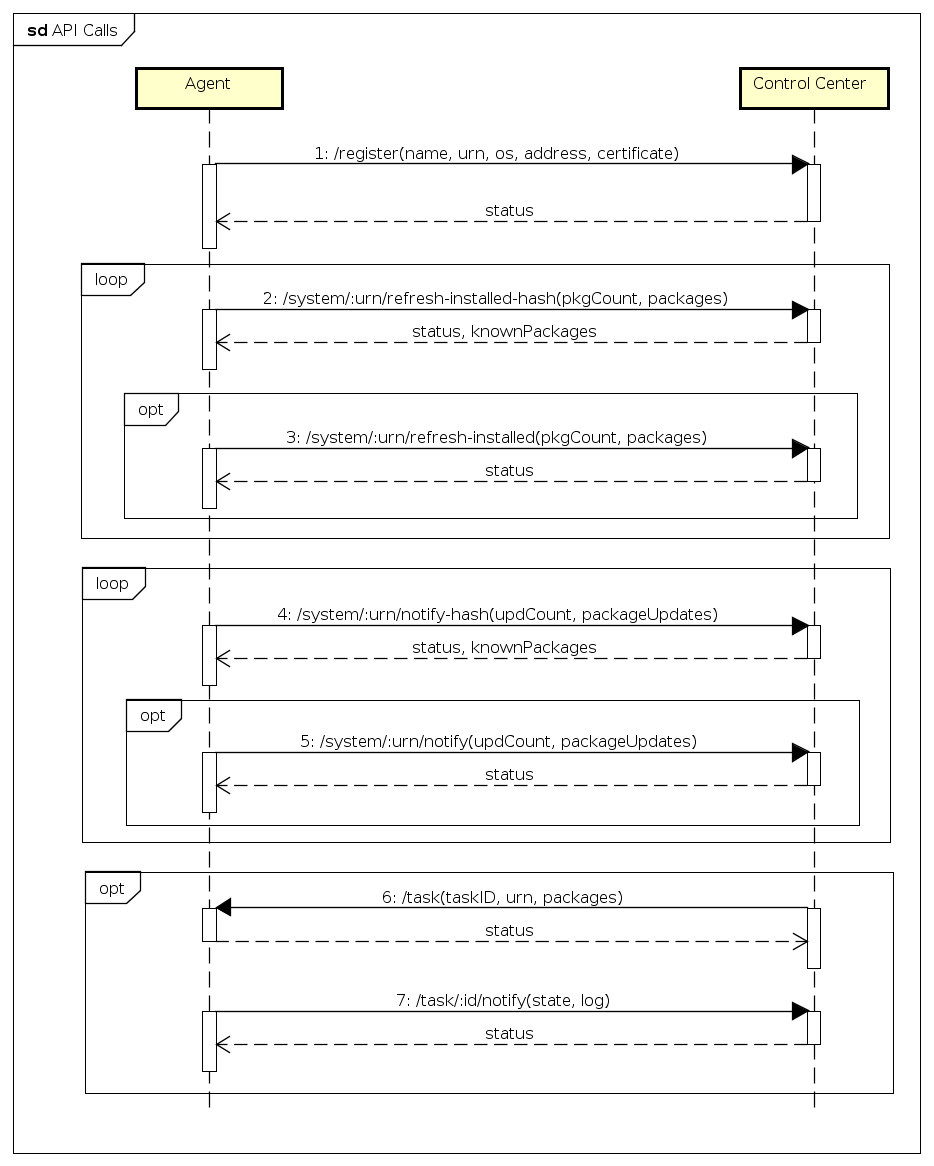
\includegraphics[width=\textwidth]{files/API_Calls}
  \caption{Sequenzdiagramm bezüglich API-Aufrufe}
  \label{fig:api_sequence_diagram}
\end{figure}

\subsubsection*{Ablauf}

Der typische Ablauf einer 'Unterhaltung' zwischen Agent und Control Center läuft folgendermassen ab (Grafisch dargestellt in Bild \ref{fig:api_sequence_diagram}):

\begin{enumerate}
    \item Registrierung: Nach dem Deployment und Start des Agents nimmt dieser Kontakt mit dem Control Center auf und registriert sich. Dazu übermittelt er seine Eckdaten wie Name, Betriebssystem und Adresse.
    \item Installierte Pakete (Hashes): Damit das Inventar beim Control Center stimmt, schickt der Agent all seine momentan installierten Pakete. Dies umfasst nicht die anstehenden Updates. Zuerst werden nur die Hash-Werte der einzelnen Paketversionen geschickt, für den Fall, dass dem Control Center bereits einige oder alle Hashes bekannt sind.
    \item Installierte Pakete (Komplett): Sollte das Control Center nicht alle gesendeten Hashes kennen, schickt der Agent die vollen Informationen.
    \item Updates (Hashes): In regelmässigen Abständen prüft der Agent über \gls{apt}, ob Updates anstehen. Ist das der Fall, übermittelt er diese (wieder zuerst nur die Hashes) an das Control Center.
    \item Updates (Komplett): Wenn Hashes unbekannt sind, meldet das Control Center dies und der Agent schickt erneut die kompletten Angaben zu den Updates.
    \item Auftrag: Sobald ein Benutzer auf dem Control Center einen Job mit einem Task für dieses System erstellt, wird dieser Task an den entsprechenden Agenten geschickt. Der Agent erhält die Version und Namen der Pakete, welche aktualisiert werden sollen, sowie eine Task-Nummer, mit welcher er den Task auf dem Control Center referenzieren kann.
    \item Feedback: Der Agent versucht, das Update über \gls{apt} auszuführen. Die Ausgaben von apt werden gesammelt und zusammen mit dem erreichten Ergebnis (Erfolgreich oder Fehlgeschlagen) zurück an das Control Center geschickt. Damit dieses weiss, um welchen Task es geht, verweist der Agent auf die vorhin erhaltene Task-Nummer.
\end{enumerate}

Punkte 2 oder 3 werden alle 2 Stunden ausgeführt, Punkte 4 und 5 alle 10 Minuten.